% vim: set spelllang=fr:
\documentclass{main}

\title{\textbf{Séance 4}\\Mathématiques}
\institute{Université de Montpellier}
\author{Mattéo Delabre, Guillaume Pérution-Kihli \& Julien Rodriguez}
\date{21 février 2021}

\begin{document}

% \begin{frame}{Programme d’entraînement}
%     \begin{itemize}
%         \item 31 janvier --- Introduction et stratégies de recherche
%         \item 7 février --- Graphes (partie 1)
%         \item 14 février --- Graphes (partie 2)
%         \item \textbf{21 février --- Mathématiques}
%         \item Semaine du 22 au 28 février --- Chaînes de caractères
%         \item Semaine du 22 au 28 février --- Géométrie algorithmique
%         \item Semaine du 22 au 28 février --- Concours blanc
%         \item 6 et 7 mars --- SWERC
%     \end{itemize}
% \end{frame}

\maketitle

\begin{frame}{Motivations}
    \begin{itemize}
        \item Dans certains problèmes, il suffit de trouver la bonne formule.
        \item Souvent autour des entiers, et souvent des formules ad-hoc.
        \item Il existe des recettes générales qui pourront vous être utiles.
    \end{itemize}
\end{frame}

\begin{frame}{Manipulation des nombres en Python}
    \begin{itemize}
        \item Pas d’entier maximal en Python (contrairement à C ou C++)
        \begin{itemize}
            \item Opérations sur les entiers en $O(1)$ seulement en dessous de \href{https://docs.python.org/3/library/sys.html\#sys.maxsize}{\texttt{sys.maxsize}} (environ $10^{18}$)
        \end{itemize}
        \item \textbf{Éviter les nombres flottants à tout prix !}
        \begin{itemize}
            \item \texttt{/} : division flottante
            \item \texttt{//} : division entière
        \end{itemize}
        \item Modules standards utiles
        \begin{itemize}
            \item \href{https://docs.python.org/3/library/math.html}{\texttt{math} : Opérations classiques (puissances, racines, arrondi, …)}
            \item \href{https://docs.python.org/3/library/fractions.html}{\texttt{fractions} : Représentation exacte des nombres rationnels (à privilégier par rapport aux flottants car pas d’arrondi)}
            \item \href{https://docs.python.org/3/library/cmath.html}{\texttt{cmath} : Équivalent de \texttt{math} pour les nombres complexes}
            \item \href{https://docs.python.org/3/library/decimal.html}{\texttt{decimal} : Flottants décimaux à précision ajustable}
        \end{itemize}
    \end{itemize}
\end{frame}

\section{Algorithme d’Euclide --- Diviseurs et multiples communs}
\maketoc

\begin{frame}{Algorithme d’Euclide}
    \begin{minipage}{\dimexpr.7\textwidth-2em}
        \begin{itemize}
            \item \(\pgcd(a, b)\) : Plus grand diviseur\\commun à deux entiers \(a\) et \(b\)
            \item \textbf{Algorithme d’Euclide :}
            \begin{enumerate}
                \item \(\pgcd(a, b) = \pgcd(b, a\bmod b)\)
                \item \(\pgcd(a, 0) = a\) \quad \emph{[si \(a \neq 0\)]}
            \end{enumerate}
        \end{itemize}
        
        \vspace*{-2.25em}
        \begin{align*}
            &\pgcd(728, 388) = \pgcd(388, 340)\\
            =\ &\pgcd(340, 48) = \pgcd(48, 4)\\
            =\ & \pgcd(4, 0) = 4
        \end{align*}
        
        \vspace*{.25em}
        \begin{itemize}
            \item Complexité : \(O(\log(a + b))\)
        \end{itemize}
    \end{minipage}\hfill%
    \begin{minipage}{.3\textwidth}
        \raggedleft
        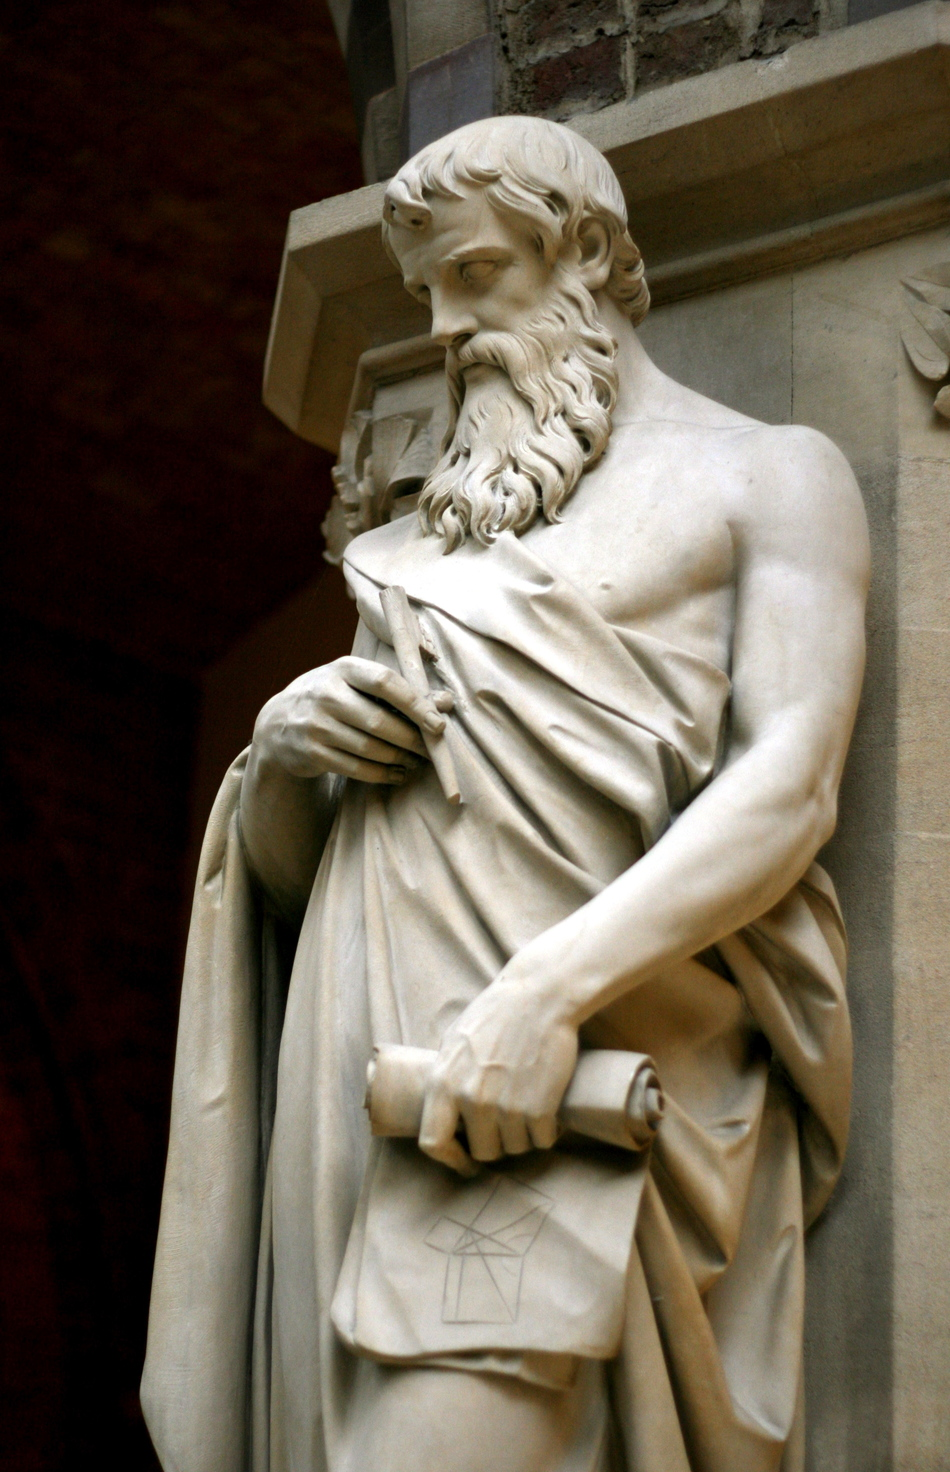
\includegraphics[width=\linewidth]{figs/euclid}
        
        \vspace{.5em}
        \tiny\itshape
        Statue d’Euclide au musée de l’Université d'Oxford --- Photographié par Mark~A.~Wilson (CC-BY-SA~4.0)
    \end{minipage}
\end{frame}

\begin{frame}[fragile]{PGCD en Python}
    \begin{itemize}
        \item Programmation de l’algorithme \emph{à la main}
    \end{itemize}
    \begin{minted}{python}
def gcd(a, b):
    while b:
        a, b = b, a % b
    return a
    \end{minted}
    \begin{itemize}
        \item En utilisant la bibliothèque standard
    \end{itemize}
    \begin{minted}{python}
>>> import math
>>> math.gcd(728, 388)
4
    \end{minted}
\end{frame}

\begin{frame}{Signaux clignotants}
    \begin{itemize}
        \item \emph{Vous apercevez deux signaux clignotants au loin. L’un s’allume toutes les 6~s et l’autre toutes les 8~s. Quel intervalle de temps faut-il pour qu’ils s’éclairent simultanément?}
    \end{itemize}
    
    \pause
    {\centering
    \begin{tikzpicture}[
        x=8pt,
        y=-1cm,
        font=\itshape\footnotesize,
        timestamp/.style={
            circle, fill,
            inner sep=3pt,
            outer sep=0pt,
        },
        >=Latex,
    ]
        \draw[->] (0, 0) -- (26, 0) node[right] {signal 1};
        \draw[->] (0, 1) -- (26, 1) node[right] {signal 2};
        \foreach \x in {0,...,24} \draw (\x, 0) -- (\x, 1);
        \foreach \x in {0,5,...,20,24} \draw (\x, 0) -- (\x, -.3)
            node[above] {\x~s};
        \foreach \x in {0,6,...,24} \node[timestamp] at (\x, 0) {};
        \foreach \x in {0,8,...,24} \node[timestamp] at (\x, 1) {};
    \end{tikzpicture}
    
    }
    
    \begin{itemize}
        \item $\ppcm(6, 8) = 24$
        \item $\ppcm(a, b)$ : Plus petit multiple commun à deux entiers $a$ et $b$
        \begin{itemize}
            \item $\ppcm(a, b) = ab / \pgcd(a, b)$
        \end{itemize}
    \end{itemize}
\end{frame}

\begin{frame}{Exercices et références}
    \begin{itemize}
        \item Exercices:
        \begin{itemize}
            \item \href{https://vjudge.net/problem/UVA-11388}{UVa 11388, “GCD LCM”}
            \item \href{https://vjudge.net/problem/UVA-10814}{UVa 10814, “Simplifying Fractions”}
        \end{itemize}
        \item Dans les livres de référence:
        \begin{itemize}
            \item Dürr et Vie, §14.1
            \item Laaksonen, §11.1.3
            \item Halim, §5.5.2
        \end{itemize}
    \end{itemize}
\end{frame}

\section{Algorithme d’Euclide étendu --- Coefficients de Bézout}
\maketoc

\begin{frame}{Problèmes d’argent}
    \begin{itemize}
        \item \emph{Vous vous trouvez dans un pays où les seules devises disponibles sont 5~¤ et 7~¤. Vous souhaitez acheter un objet qui coûte 1~¤. Comment faire ?\quad\footnotesize Indice: On peut vous rendre de la monnaie}
    \end{itemize}
    
    \pause
    {\centering
    \begin{tikzpicture}[>=Latex]
        \node[outer sep=8pt] (vous) at (-3, 0){Vous};
        \node[outer sep=8pt] (vend) at (3, 0) {Vendeur};
        \node (sum) {
            \only<8->{\bfseries}
            \rmfamily{\footnotesize total:}
            \strut\only<2>{0}\only<3>{7}\only<4>{2}\only<5>{9}\only<6>{4}\only<7>{11}\only<8->{1}
        };
        
        \draw[->] (vous) to[bend left=20] 
            node[above] {\footnotesize\strut\only<3->{7}\only<5->{ + 7}\only<7->{ + 7}}
            (vend);
            
        \draw[->] (vend) to[bend left=20]
            node[below] {\footnotesize\strut\only<4->{5}\only<6->{ + 5}\only<8->{ + 5 + 5}}
            (vous);
    \end{tikzpicture}
    
    }
    
    \onslide<8->{
    \begin{itemize}
        \item Puisqu’on peut payer 1~¤, on peut payer n’importe quel montant !
        \item Est-ce vrai pour des devises de valeur 4~¤ et 6~¤ ?
    \end{itemize}
    }
\end{frame}

\begin{frame}{Identité de Bézout}
    \begin{itemize}
        \item Nous cherchions en fait des solutions entières à l’équation suivante, où $x$ et $y$ sont des entiers relatifs (le nombre de devises échangées)
    \end{itemize}
    \vspace{-.5em}
    \[\only<1>{5}\only<2->{a}x + \only<1>{7}\only<2->{b}y = \only<1>{1}\only<2->{c}\]
    \pause
    \vspace{-2em}
    \begin{itemize}
        \item Cette forme générale est appelée \emph{identité de Bézout}
        \begin{itemize}
            \item $x$ et $y$ sont des \emph{coefficients de Bézout}
        \end{itemize}
        \item \textbf{Théorème:} Il existe des solutions \emph{si et seulement}\\\emph{si} $c$ est un multiple de $\pgcd(a, b)$
        \begin{itemize}
            \item 5x + 7y = 1 $\leadsto$ $\exists$ solutions car $\pgcd(5, 7) = 1$
            \item 4x + 6y = 1 $\leadsto$ pas de sol. car $\pgcd(4, 6) = 2$
        \end{itemize}
    \end{itemize}
\end{frame}

\begin{frame}{Algorithme d’Euclide étendu}
    \begin{minipage}{\dimexpr.7\textwidth-2em}
        \begin{itemize}
            \item Résoudre \(899x + 493y = 29\)
            \item Notons $a = 899, b = 493$ et $c = 29$
        \end{itemize}
    
        \vspace{-1em}
        \begin{align*}
        \only<1-6>{
            \only<1-5>{899}\only<6->{a}
                &= \only<1-5>{493}\only<6->{b}
                \times 1 + 406 \\
            \onslide<2->{
                \only<1-5>{493}\only<6->{b}
                &= 406 \times 1 + 87} \\
            \onslide<3->{406 &= 87 \times 4 + 58} \\
            \onslide<4->{87 &= 58 \times 1
                + \only<4-5>{29}\only<6->{c}} \\
            \onslide<5>{58 &= 29 \times 2 + 0} \\
        }\only<7->{
            \only<8,10->{406}\only<7,9>{\textbf{406}} &= a - b \times 1\\
            \only<7,8,10,12->{87}\only<9,11>{\textbf{87}} &= \only<7-8>{
                b - \only<7>{\textbf{406}}\only<8>{(a - b \times 1)} \times 1
            }\only<9->{
                -a + b \times 2
            }\\
            \only<7-10,12->{58}\only<11>{\textbf{58}} &= \only<7-10>{
                \only<7-8>{406}\only<9>{\textbf{406}}\only<10>{(a - b \times 1)}
                - \only<7-8>{87}\only<9>{\textbf{87}}\only<10>{(-a + b \times 2)} \times 4
            }\only<11->{
                a \times 5 - b \times 9
            }\\
            c &= \only<7-12>{
                \only<7-10>{87}\only<11>{\textbf{87}}\only<12>{(-a + b \times 2)}
                - \only<7-10>{58}\only<11>{\textbf{58}}\only<12>{(a \times 5 - b \times 9)} \times 1
            }\only<13->{
                -a \times 6 + b \times 11
            }\\
            \phantom{-}\\
        }
        \end{align*}
        \onslide<13->{
        \vspace*{-3.5em}
        \begin{itemize}
            \item Solution : \(x = -6, y = 11\)
            \item Complexité : \(O(\log(a + b))\)
        \end{itemize}
        }
    \end{minipage}\hfill%
    \begin{minipage}{.3\textwidth}
        \raggedleft
        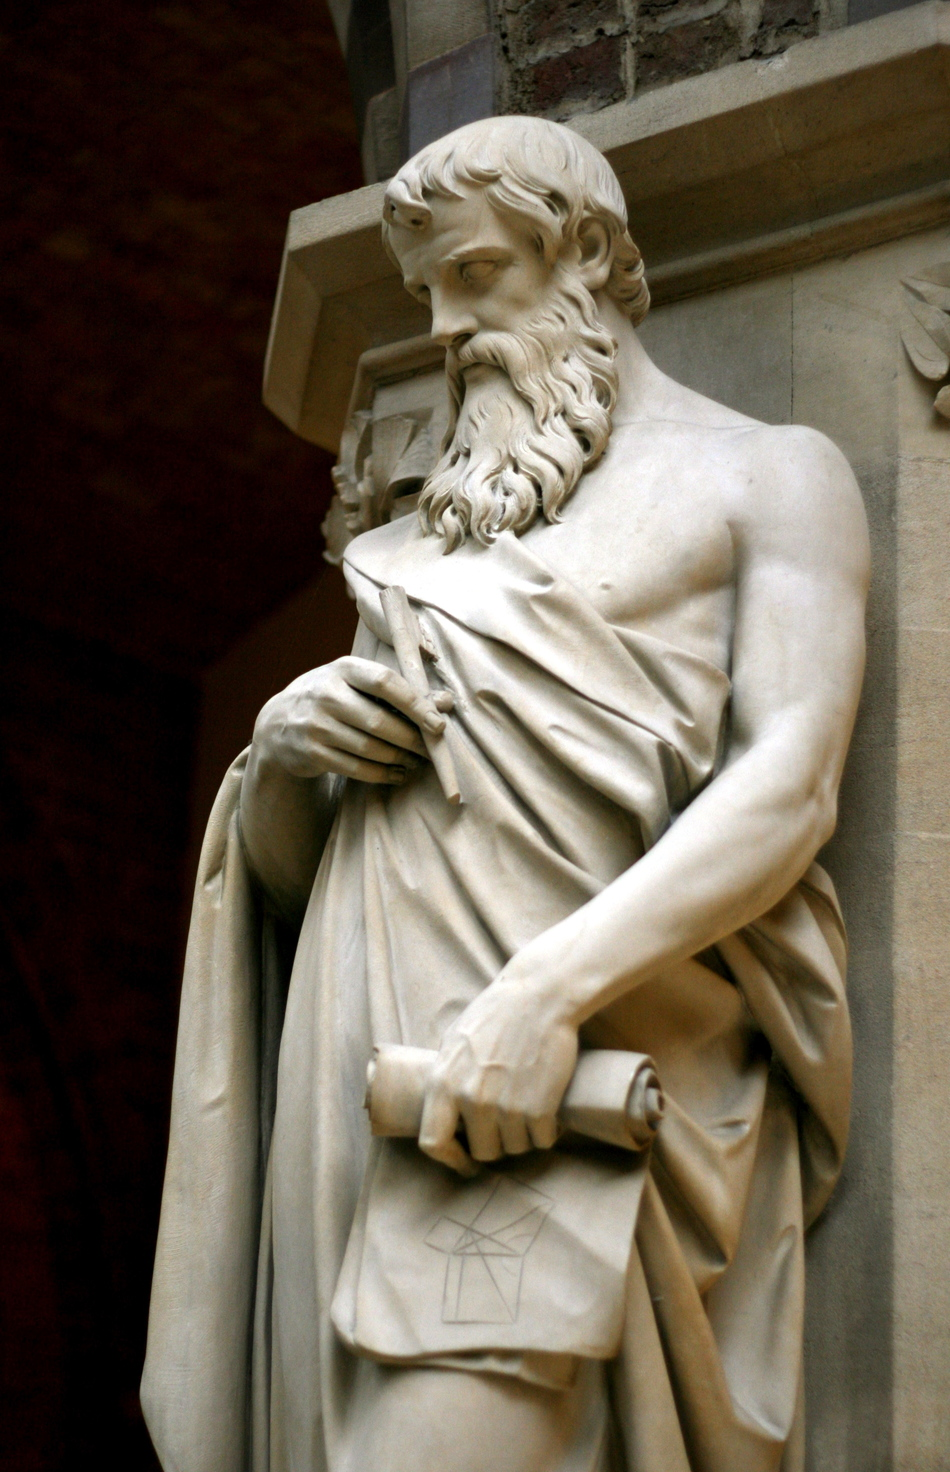
\includegraphics[width=\linewidth]{figs/euclid}
        
        \vspace{.5em}
        \tiny\itshape
        Statue d’Euclide au musée de l’Université d'Oxford --- Photographié par Mark~A.~Wilson (CC-BY-SA~4.0)
    \end{minipage}
    \begin{tikzpicture}[remember picture, overlay]
        \node[
            xshift=-2cm,
            yshift=-.8cm,
            draw, red, very thick, starburst,
            fill=yellow, rotate=10, align=center,
            font=\rmfamily,
        ] at (current page.east) {2 en 1 !};
    \end{tikzpicture}
\end{frame}

\setlength{\fboxsep}{0pt}
\begin{frame}[fragile]{Coefficients de Bézout en Python}
    \begin{minted}[escapeinside=||]{python}
def bezout(a, b):
    |\colorbox{yellow}{px, py = 1, 0}|
    |\colorbox{yellow}{x, y = 0, 1}|
    while b:
        a, b|\colorbox{yellow}{, q}| = b, a % b|\colorbox{yellow}{, a // b}|
        |\colorbox{yellow}{px, py, x, y = x, y, px - q * x, py - q * y}|
    return a|\colorbox{yellow}{, px, py}|
    \end{minted}
\end{frame}

\begin{frame}{Exercices et références}
    \begin{itemize}
        \item Exercices:
        \begin{itemize}
            \item \href{https://vjudge.net/problem/CodeForces-633A}{Codeforces 633A, “Ebony and Ivory”}
            \item \href{https://vjudge.net/problem/UVA-10090}{UVa 10090, “Marbles”}
        \end{itemize}
        \item Dans les livres de référence:
        \begin{itemize}
            \item Dürr et Vie, §14.2
            \item Laaksonen, §11.1.6
            \item Halim, §5.5.9
        \end{itemize}
    \end{itemize}
\end{frame}

\section{Arithmétique modulaire et théorème des restes chinois}
\maketoc

\begin{frame}{Arithmétique modulaire}
    \begin{itemize}
        \item Système dans lequel on revient à 0 dès qu’on atteint un $n$ fixé.
    \end{itemize}
    
    {\centering
    \begin{tikzpicture}[
        number line/.style={very thick},
        number value/.style={font=\footnotesize},
    ]
        \draw [
            number line,
            decoration={
                markings,
                mark=at position .29 with {\arrow{Latex[reversed]}}
            },
            postaction={decorate},
        ] (0, 0) circle (1);
        
        \foreach[
            evaluate=\number as \angle using int(90-\number*360/10)
        ] \number in {0,...,9} {
            \draw[number line] (\angle:0.9) -- (\angle:1.1);
            \node[number value] at (\angle:1.3) {\number};
        };
    \end{tikzpicture}
    
    }
    
    \begin{itemize}
        \item Permet de faire des calculs sur des nombres de taille bornée.
        \item Souvent utilisée dans les problèmes mathématiques des concours.
    \end{itemize}
\end{frame}

\begin{frame}{Quelques règles du modulo}
    \begin{itemize}
        \item L’opérateur modulo est linéaire et se comporte\\intuitivement la plupart du temps.
        \vspace{1em}
        \item \emph{Addition}
        \begin{itemize}
            \item \(
                a + b = c
                \Rightarrow (a \bmod n) + (b \bmod n) \equiv c \pmod{n}
            \)
            \item \(
                a \equiv b \pmod{n}
                \Rightarrow a + k \equiv b + k \pmod{n}
            \)
            \item \(
                a \equiv b \pmod{n} \land c \equiv d \pmod{n}
                \Rightarrow a + c \equiv b + d \pmod{n}
            \)
        \end{itemize}
        \item \emph{Multiplication}
        \begin{itemize}
            \item \(
                a \times b = c
                \Rightarrow (a \bmod n) \times (b \bmod n) \equiv c \pmod{n}
            \)
            \item \(
                a \equiv b \pmod{n}
                \Rightarrow ka \equiv kb \pmod{n}
            \)
            \item \(
                a \equiv b \pmod{n} \land c \equiv d \pmod{n}
                \Rightarrow ac \equiv bd \pmod{n}
            \)
        \end{itemize}
        \item \emph{Exponentiation}
        \begin{itemize}
            \item \(
                a \equiv b \pmod{n}
                \Rightarrow a^k \equiv b^k \pmod{n}
                \quad [k \geq 0]
            \)
        \end{itemize}
    \end{itemize}
\end{frame}

\begin{frame}{Inverse modulaire}
    \begin{itemize}
        \item Qu’est-ce que l’inverse d’un nombre $a$ ?
        \begin{itemize}
            \pause
            \item Sur les rationnels et les réels, l’inverse de $a$ est $1 / a$
            \pause
            \item Un nombre $x$ qui \enquote{annule} l’effet multiplicatif de $a$
            \pause
            \item Une solution à l’équation $ax = 1$
        \end{itemize}
        \item En arithmétique modulaire, les nombres ont des inverses entiers!
        \begin{itemize}
            \item Ex: Pour un module $n = 20$, $7$ est l’inverse de $3$\\
                \quad\quad$7 \times 3 = 21 \equiv 1 \pmod{20}$
            \item Comment trouver l’inverse de $a$ modulo $n$ ?
            \pause
            \begin{align*}
                ax &\equiv 1 \pmod{n}\\
                ax + qn &= 1 \quad\leadsto \text{identité de Bézout !}\\
            \end{align*}
        \end{itemize}
    \end{itemize}
\end{frame}

\begin{frame}[fragile]{Inverse modulaire en Python}
    \begin{minted}{python}
def inv(a, n):
    gcd, inv, _ = bezout(a, n)
    if gcd != 1:
        return None
    return inv % n
    \end{minted}
\end{frame}

\invert{
\begin{frame}{Bio-rythmes}
    \small
    \vspace{-\parskip}
    \begin{minipage}[t]{\dimexpr\linewidth-3cm-2em}
        \vspace*{0pt}
        Trois cycles courent en parallèle chez une personne : \emph{physique}, \emph{émotionnel} et \emph{intellectuel}.
        Ils atteignent un pic respectivement tous les 23, 28 et 33~jours.
        Sachant le numéro de trois jours où se sont produits des pics pour chacun des trois cycles, ainsi que le numéro du jour actuel, dans combien de jours se produira le prochain pic simultané ?
    \end{minipage}\hfill%
    \begin{minipage}[t]{3cm}
        \vspace*{0pt}
        \raggedleft
        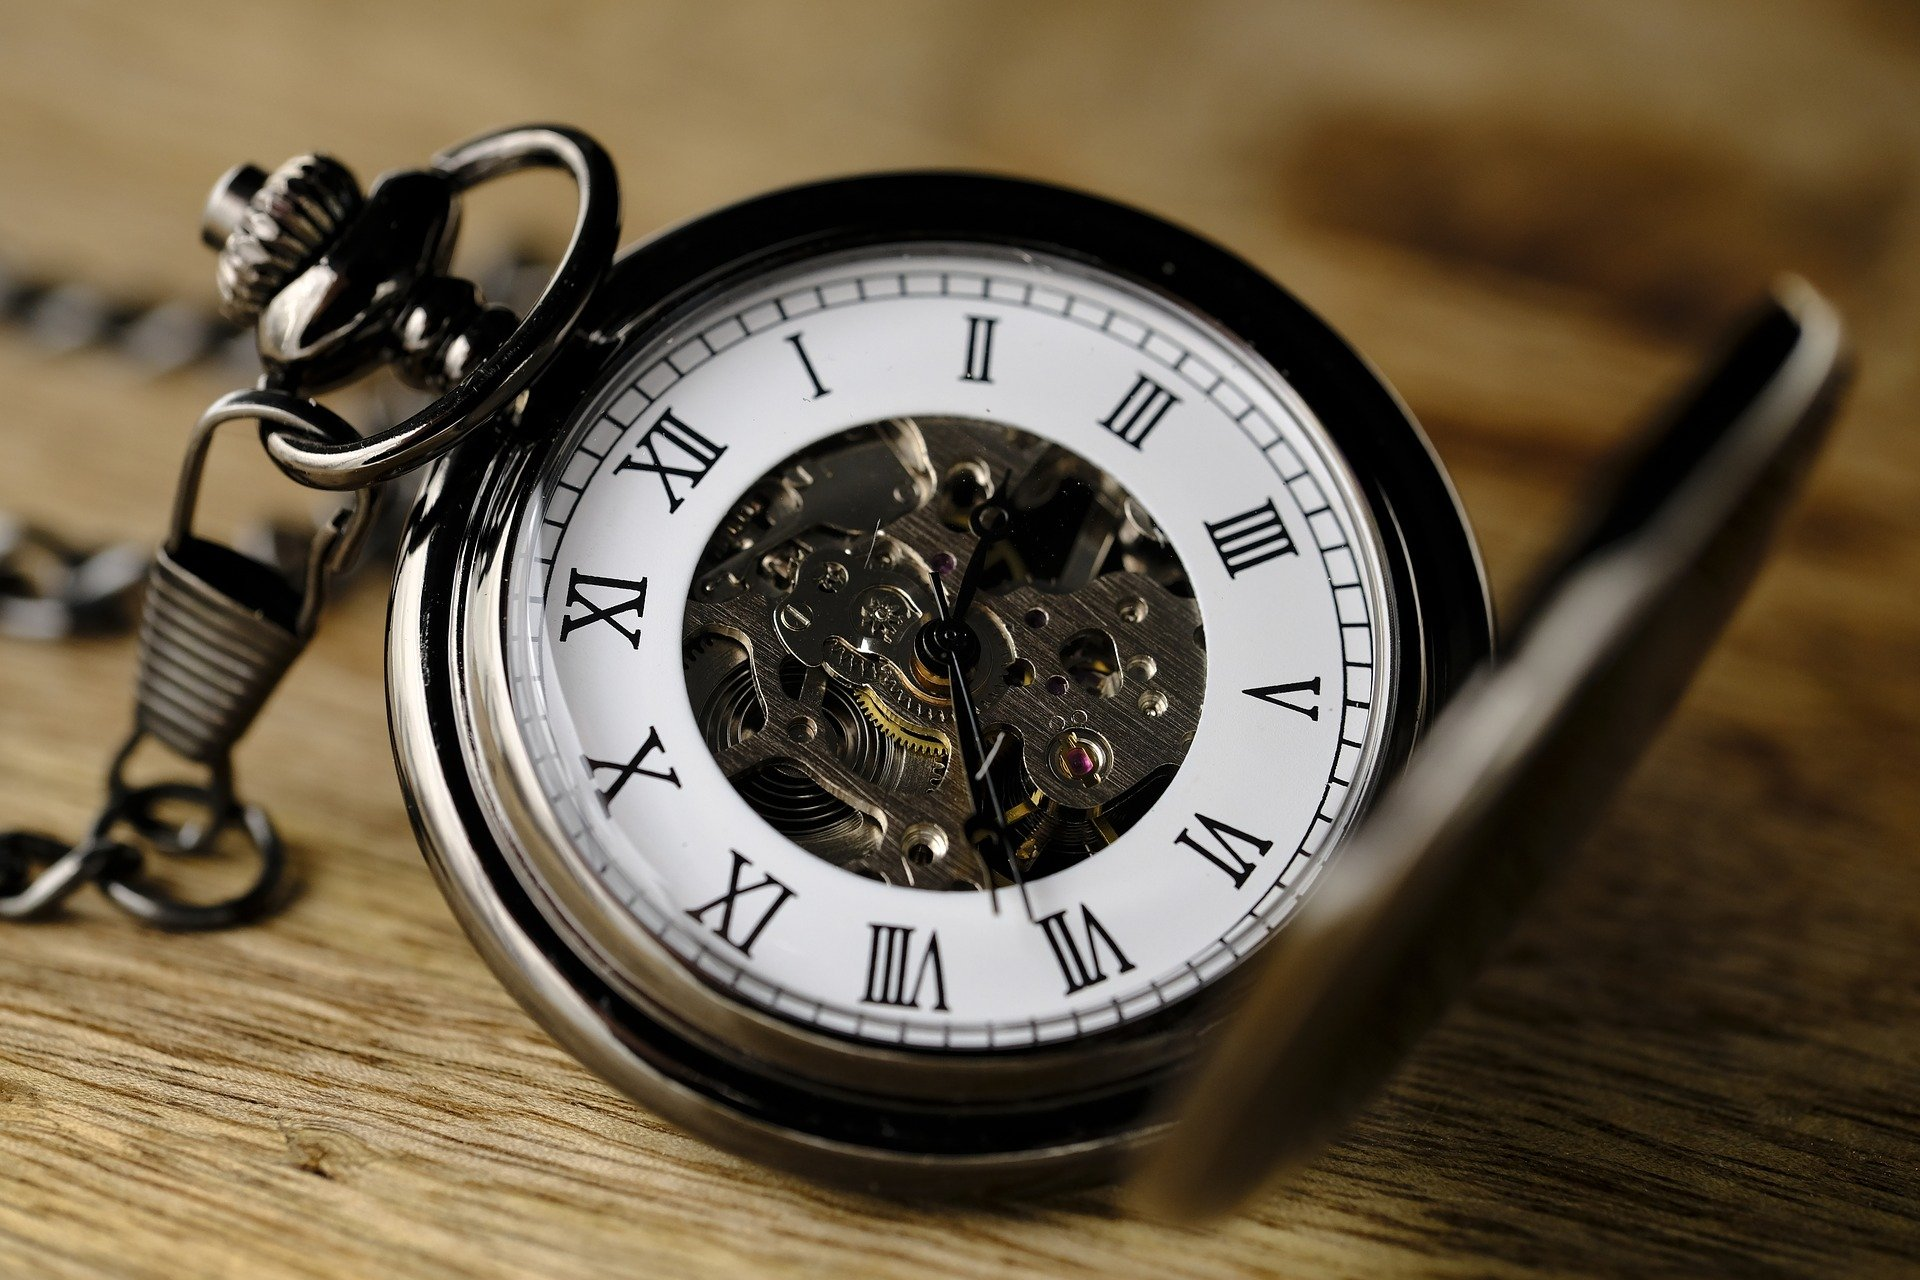
\includegraphics[width=\linewidth]{figs/clock}
    \end{minipage}
    
    \textbf{Entrée}\quad
    Quatre entiers $p$, $e$, $i$ et $d$, les numéros des jours où se sont produits les pics des trois types et le numéro du jour actuel.
    
    \textbf{Limites}\quad
    \(0 \leq p, e, i, d \leq 365\).
    Temps: 3~s.
    
    \textbf{Sortie}\quad
    \enquote{the next triple peak occurs in $x$ days.}, où $x$ est votre réponse.
    
    \vspace{1em}
    \scriptsize\emph{Tiré de UVa~756, “Biorhythms”} 
\end{frame}
}

\begin{frame}{Pensez modulo}
    \begin{itemize}
        \item Pouvez-vous reformuler le problème en arithmétique modulaire ?
        \pause
        \item Si $k$ est le numéro d’un jour de triple-pic, il vérifie les équations
    \end{itemize}
    \[\begin{cases}
        &k \equiv p \pmod{23}\\
        &k \equiv e \pmod{28}\\
        &k \equiv i \pmod{33}\\
    \end{cases}\]
    \vspace{-1em}
    \begin{itemize}
        \item Le \textbf{théorème des restes chinois} nous permet de résoudre les systèmes d’équations de cette forme
    \end{itemize}
\end{frame}

\begin{frame}{Théorème des restes chinois}
    \begin{itemize}
        \item Soit un système d’équations modulaires de la forme
        \[\begin{cases}
            &x \equiv a_1 \pmod{n_1}\\
            &\vdots\\
            &x \equiv a_k \pmod{n_k}\\
        \end{cases}\]
        \item Si $n_1, ..., n_k$ sont premiers entre eux, une solution est
        \begin{align*}
            x &=
                a_1\,X_1\,\inv_{n_1}(X_1) + \cdots
                + a_k\,X_k\,\inv_{n_k}(X_k)\\
            \text{où\enspace}X_i &= (n_1 \times \cdots \times n_k) / n_i
        \end{align*}
        \item D’autres solutions obtenues en ajoutant ou retranchant $n_1 \times \cdots \times n_k$
    \end{itemize}
    \vspace{-1em}
\end{frame}

\begin{frame}[fragile]{Théorème des restes chinois en Python}
    \begin{minted}{python}
from math import prod
def crt(a, n):
    x = 0
    p = prod(n)
    for ai, ni in zip(a, n):
        xi = p // ni
        x += ai * xi * inv(xi, ni)
    return x
    \end{minted}
\end{frame}

\begin{frame}{Exercices et références}
    \begin{itemize}
        \item Exercices:
        \begin{itemize}
            \item \href{https://adventofcode.com/2020/day/13}{AoC 2020-13, “Shuttle Search”}
            \item \href{https://onlinejudge.org/index.php?option=onlinejudge&Itemid=8&page=show_problem&problem=697}{\textbf{UVa 756, “Biorhythms”}}
        \end{itemize}
        \item Dans les livres de référence:
        \begin{itemize}
            \item Laaksonen, §11.1.6
        \end{itemize}
    \end{itemize}
\end{frame}


\section{Nombres de Catalan}
\maketoc

\begin{frame}{Nombres de Catalan}
\vspace{-25pt}
\[
    C_n = \frac{1}{n+1}{2n\choose n} = \frac{(2n)!}{(n+1)!\,n!} = \prod\limits_{k=2}^{n}\frac{n+k}{k} \qquad\mbox{ pour }n\ge 0.
\]
\vspace{-15pt}
Liste non-exhaustive : 
\begin{itemize}
    \item Nombre de mots de Dyck de longueur $2n$
    \item Nombre d'arbres binaires entiers à $n + 1$ feuilles
    \item Nombre d'arbres planaires enracinés à $n$ arêtes
    \item ...
\end{itemize}

\begin{itemize}
    \item Pas possible de tout retenir, il faut utiliser votre plaquette SWERC 
    \item Exercice : \href{https://cses.fi/problemset/task/2064}{\textbf{Bracket Sequences I}} \\
\visible<2>{    \item Plus de détails et de problèmes : \href{https://codeforces.com/blog/entry/87585}{[Tutorial] Catalan Numbers and Catalan Convolution}}
\end{itemize}
\end{frame}

\section{Pivot de Gauss}
\maketoc

\begin{frame}{Pivot de Gauss}
\vspace{-15pt}
On veut déterminer les solutions d'un système d'équations linéaires à $n$ variables :
\vspace{-15pt}
    \begin{alignat}{5}
  a_{1,1}x_1 &{}+{}& a_{1,2}x_2 &{}+{}& \dots & {}+{} &  a_{1,n}x_n &{}={}& b_1   \\
  a_{2,1}x_1 &{}+{}& a_{2,2}x_2 &{}+{}& \dots & {}+{} &  a_{2,n}x_n &{}={}& b_2   \\
  \dots \\ 
  a_{n,1}x_1 &{}+{}& a_{n,2}x_2 &{}+{}& \dots & {}+{} &  a_{n,n}x_n &{}={}& b_n   
\end{alignat}
Représentation en matrice :
$$\left[\begin{array}{rrrr|r}
  a_{1,1} &  a_{1,2} & \dots &   a_{1,n} & b_1 \\
  a_{2,1} &  a_{2,2} & \dots &   a_{1,n} & b_2 \\
  \vdots &  \vdots & \ddots &   \vdots  & \vdots \\
  a_{n,1} &  a_{n,2} & \dots &   a_{n,n} & b_n \\
\end{array}\right]$$
\end{frame}


\begin{frame}{Pivot de Gauss}
Pour résoudre le système, on veut transformer la matrice :
$$\left[\begin{array}{rrrr|r}
  a_{1,1} &  a_{1,2} & \dots &   a_{1,n} & b_1 \\
  a_{2,1} &  a_{2,2} & \dots &   a_{1,n} & b_2 \\
  \vdots &  \vdots & \ddots &   \vdots  & \vdots \\
  a_{n,1} &  a_{n,2} & \dots &   a_{n,n} & b_n \\
\end{array}\right]$$
En : 
$$\left[\begin{array}{rrrr|r}
  1 &  0 & \dots &   0 & c_1 \\
  0 &  1 & \dots &   0 & c_2 \\
  \vdots &  \vdots & \ddots &   \vdots  & \vdots \\
  0 &  0 & \dots &   1 & c_n \\ 
\end{array}\right]$$
\end{frame}

\begin{frame}{Pivot de Gauss}
Pour l'échelonnement, trois types d'opérations :
\begin{itemize}
    \item     Échange de deux lignes
    \item     Multiplication d'une ligne par un scalaire non nul
    \item     Ajout du multiple d'une ligne à une autre ligne
\end{itemize}
\centering
\only<1>{Exercice : résoudre le système d'équations
    \begin{alignat}{4}
  2x_1 &{}+{}& 4x_2 &{}+{}& x_3 &{}={}& 16   \\
  x_1 &{}+{}& 2x_2 &{}+{}& 5x_3 &{}={}& 17   \\
  3x_1 &{}+{}& x_2 &{}+{}& x_3 &{}={}& 8   
\end{alignat}
}
\only<2>{Exercice : résoudre le système d'équations 
    \begin{tabular}{c|c}
$$\left[\begin{array}{rrr|r}
  2 &  4 & 1 & 16 \\ 
  1 &  2 & 5 & 17 \\ 
  3 &  1 & 1 & 8 \\ 
\end{array}\right]$$ 
         &  
$$\left[\begin{array}{rrr|r}
  1 &  0 & 0 & 1 \\ 
  0 & 1  & 0 & 3 \\ 
  0 &  0 & 1 & 2 \\ 
\end{array}\right]$$
    \end{tabular} \\
   ~~~~~~~ Matrice en entrée / Matrice échelonnée
}
\only<3>{Ces 3 opérations sont utilisées pour réaliser l'algorithme de Gauss-Jordan (complexité $O(n^3)$) : \\ {\small \url{https://github.com/jilljenn/tryalgo/blob/master/tryalgo/gauss\_jordan.py}} \\[4pt]
\centering Exercice : \href{https://vjudge.net/problem/Gym-100923C}{Por Costel and Bujor}

}
\end{frame}

\end{document}